\documentclass[11pt,letterpaper]{exam}
%\usepackage[Lhdr={},Rhdr={}]{plain}

\newtheorem{proposition}{Proposition}
\newcommand{\blue}[1]{\textcolor{blue}{#1}}
\newcommand{\white}[1]{\textcolor{white}{#1}}

\usepackage{tikz}
\usetikzlibrary{shapes.geometric}
\usepackage{pgfplots}
\usetikzlibrary{patterns, pgfplots.fillbetween}
\usepackage{graphicx}
\usepackage{verbatim}
\usepackage{subfigure}
\usetikzlibrary{positioning}
\usetikzlibrary{snakes}
\usetikzlibrary{calc}
\usetikzlibrary{arrows}
\usetikzlibrary{decorations.markings}
\usetikzlibrary{shapes.misc}
\usetikzlibrary{matrix,shapes,arrows,fit,tikzmark}
\usepackage{amsmath}
\usepackage{mathpazo}
\usepackage{hyperref}
\usepackage{lipsum}
\usepackage{multimedia}
\usepackage{graphicx}
\usepackage{multirow}
\usepackage{graphicx}
\usepackage{dcolumn}
\usepackage{bbm}
\usepackage{comment}
 \usepackage{booktabs}
\usepackage{tabularx}
\usepackage{adjustbox}
\usepackage{graphicx}
\usepackage{multicol}
\usepackage{mathtools}
\usepackage[table,xcdraw]{xcolor}
\usepackage[top=0.5in,
  headsep=0pt% remove space between header and text body
  ]{geometry}
\usepackage{lastpage}
\cfoot{Page \thepage \hspace{1pt} of \pageref{LastPage}}

\newcommand{\figpath}{figs/}

\usepackage{titlesec}
\titleformat*{\section}{\large\bfseries}

\begin{document}
\begin{center}
\Large{\textsc{International Trade Theory and Policy}}\\[4pt]
\Large{ECON 2181 \;--\; Fall 2025}\\[6pt]
\large Carlos Góes, Ph.D. \\
\textit{Professorial Lecturer}\\
\href{mailto:c.bezerradegoes@gwu.edu}{c.bezerradegoes@gwu.edu} \\
\end{center}

\bigskip

\begin{center}
\Large{\textsc{Problem Set 3}}
\end{center}

\begin{questions}

%%%%%%%%%%%%%%%%%%%%%%%%%%%%%%%%%%%%
\question Consider a world with two countries $i \in \{H, F\}$ and two sectors: agriculture ($A$) and manufacturing ($M$). In each country, there are three factors of production: labor ($L$), land ($T$), and capital ($K$). Labor is mobile between sectors, but $T$ is specific to agriculture and $K$ is specific to manufacturing. 

The production functions are Cobb-Douglas:
\[
Y_{i,M} = Z_{i,M} K_i^{\beta_i} L_{i,M}^{1-\beta_i}, \qquad Y_{i,A} = Z_{i,A} T_i^{\beta_i} L_{i,A}^{1-\beta_i}
\]
with total labor constraint $L_{i,A} + L_{i,M} = \bar{L}_i$.

\begin{parts}

\part Draw a four quadrant diagram characterizing this economy within a given country $i$. Draw it according to the following instructions. \textcolor{brown}{Southwest: labor endowment constraint, the maximum allocation choices of labor $\bar{L}_i = L_{i,A} + L_{i,M}$}; \textcolor{blue}{Southeast: production function for agriculture as a function of labor input $Y_{i,A} = Z_{i,A} T_{i}^{\beta_i} L_{i,A}^{1-\beta_i}$}; \textcolor{black}{Northwest: production function for manufacturing as a function of labor input $Y_{i,M} = Z_{i,M} K_{i}^{\beta_i} L_{i,M}^{1-\beta_i}$}; \textcolor{red}{Northeast: production possibilities frontier $Y_{i} = Y_{i,A} + Y_{i,M}$.}


\begin{figure}[htp]
    \centering
    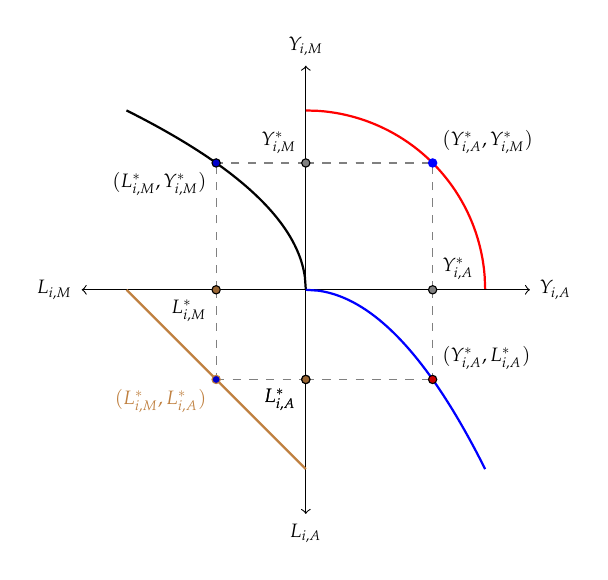
\begin{tikzpicture}
    \begin{axis}[
        axis lines=middle,
        xmin=-1.25, xmax=1.25,
        ymin=-1.25, ymax=1.25,
    %    xlabel={\small Output of cloth / Labor in cloth},
    %    ylabel={\small Output of food / Labor in food},
        xtick=\empty,
        ytick=\empty,
        axis line style={<->},
        clip=false,
        enlargelimits=false,
        domain=0.0:1,
        width=0.6\textwidth,
        height=0.6\textwidth,
        samples=200
    ]
    
    \pgfmathsetmacro{\a}{0.5}       % curvature parameter
    
    % NW: Production function for food (plot in 2nd quadrant)
    \addplot[black, thick] ({-x}, {x^(\a)});
    \node[anchor=east] at (axis cs:-1.25,0) {\scriptsize $L_{i,M}$};
    \node[anchor=south] at (axis cs:0,1.25) {\scriptsize $Y_{i,M}$};
    
    % SW: Labor allocation AA curve (line in 3rd quadrant)
    \addplot[brown, thick] ({-x}, {-1 + x});
    %\node[anchor=north east] at (axis cs:-0.95,-0.05) {\scriptsize Economy's allocation of labor (AA)};
    
    % SE: Production function for cloth (4th quadrant)
    \addplot[blue, thick] ({x^(\a)}, {-x});
    \node[anchor=west] at (axis cs:1.25,0) {\scriptsize $Y_{i,A}$};
    \node[anchor=north] at (axis cs:0,-1.25) {\scriptsize $L_{i,A}$};
    %\node[anchor=north west] at (axis cs:0.6,-0.6) {\scriptsize Production function for cloth};
    
    % NE: Production Possibility Frontier (PPF)
    \addplot[red, thick] ({x^(\a)}, {(1 - x)^(\a)});
    %\node[anchor=south east, blue] at (axis cs:0.6,0.65) {\scriptsize $PP$};
    
    % point on AA
    \addplot+[mark=*,only marks,mark size=1.5pt,brown]
                  coordinates {({-0.5},{-1+0.5})}
                  node[anchor=north east,font=\scriptsize, brown] {$(L_{i,M}^*,L_{i,A}^*)$};
    
    \addplot[dashed, gray] coordinates {({-0.5}, {-1 + 0.5}) (0, {-1 + 0.5})};

    \addplot+[mark=*,only marks,mark size=1.5pt,black]
                  coordinates {({-0.5}, 0)}
                  node[anchor=north east,font=\scriptsize] {$L_{i,M}^*$};

        \addplot+[mark=*,only marks,mark size=1.5pt,black]
                  coordinates {(0, {0.5^(\a)})}
                  node[anchor=south east,font=\scriptsize] {$Y_{i,M}^*$};

    % Project to NW (Food PF)
    \addplot[dashed, gray] coordinates {({-0.5}, 0) ({-0.5}, {0.5^(\a)})};
    \addplot[dashed, gray] coordinates {(0, {0.5^(\a)}) ({-0.5},{0.5^(\a)})};
    \addplot+[mark=*, only marks, mark size=1.5pt, black]
            coordinates {({-0.5}, {0.5^(\a)})}
            node[anchor=north east, font=\scriptsize]{$(L_{i,M}^*,Y_{i,M}^*)$};     

    \addplot[dashed, gray] coordinates {({-0.5}, 0) ({-0.5}, {-(1-0.5)})};
    \addplot+[mark=*,only marks,mark size=1.5pt,black]
                  coordinates { (0, {-(1-0.5)})}
                  node[anchor=north east,font=\scriptsize] {$L_{i,A}^*$};

        % Project to SE (Cloth PF)
    \addplot[dashed, gray] coordinates {(0, {-0.5}) ({0.5^(\a)}, {-0.5})};
    \addplot[dashed, gray] coordinates {({0.5^(\a)}, 0) ({0.5^(\a)}, {-0.5})};
    \addplot+[mark=*, only marks, mark size=1.5pt, black]
            coordinates {({0.5^(\a)}, {-0.5})}
            node[anchor=south west,font=\scriptsize] {$(Y_{i,A}^*,L_{i,A}^*)$};
    
    \addplot+[mark=*,only marks,mark size=1.5pt,black]
                  coordinates { (0, {-(1-0.5)})}
                  node[anchor=north east,font=\scriptsize] {$L_{i,A}^*$};

        \addplot+[mark=*,only marks,mark size=1.5pt,black]
                  coordinates {({0.5^(\a)},0)}
                  node[anchor=south west,font=\scriptsize] {$Y_{i,A}^*$};


    % Project to NE (PPF)
    \pgfmathsetmacro{\Qc}{0.5^(\a)}
    \pgfmathsetmacro{\Qf}{(1 - 0.5)^(\a)}
    \addplot+[mark=*, only marks, mark size=1.5pt]
            coordinates {(\Qc, \Qf)}
            node[anchor=south west, font=\scriptsize, black]{$(Y_{i,A}^*,Y_{i,M}^*)$};     
    \addplot[dashed, gray] coordinates {(\Qc, 0) (\Qc, \Qf)};
    \addplot[dashed, gray] coordinates {(0, \Qf) (\Qc, \Qf)};
    \addplot[dashed, gray] coordinates {(0, \Qf) (\Qc, \Qf)};

    
    \end{axis}
    
    \end{tikzpicture}
    \end{figure}

\part Why do the production functions are belly shaped (concave)? What is the economic concept that relates to that shape?

    \textcolor{red}{The "belly shaped" (concave) function relates to diminishing marginal returns. As you hold $K,T$ fixed an increase $L$, each additional worker adds less to output, because MPL is decreasing in labor.}


\part Write down the profit maximization problem for a representative firm in each sector in country $i$, taking as given factor prices $w_i, r_{i,M}, r_{i,A}$ and output prices $P_M, P_A$.

\textcolor{red}{
Manufacturing:
\[
\max_{L_{i,M}, K_i} P_M Z_{i,M} K_i^{\beta_i} L_{i,M}^{1-\beta_i} - w_i L_{i,M} - r_{i,M} K_i
\]
Agriculture:
\[
\max_{L_{i,A}, T_i} P_A Z_{i,A} T_i^{\beta_i} L_{i,A}^{1-\beta_i} - w_i L_{i,A} - r_{i,A} T_i
\]
}

\part Derive the first-order conditions with respect to each choice variable. What do they imply about wages and returns to specific factors?

\textcolor{red}{
For labor:
\[
P_M Z_{i,M} (1-\beta_i) K_i^{\beta_i} L_{i,M}^{-\beta_i} = P_M \times MPL_{i,M} = w_i
\]
\[
P_A Z_{i,A} (1-\beta_i) T_i^{\beta_i} L_{i,A}^{-\beta_i} = P_A \times MPL_{i,A} = w_i
\]
For capital:
\[
P_M Z_{i,M} \beta_i K_i^{\beta_i-1} L_{i,M}^{1-\beta_i} = P_M \times MPK_{i,M} = r_{i,M}
\]
For land:
\[
P_A Z_{i,A} \beta_i T_i^{\beta_i-1} L_{i,A}^{1-\beta_i} = P_A \times MPT_{i,A} = r_{i,A}
\]
Interpretation: In equilibrium, each factor's price equals its marginal revenue product.
}

\part How does the equilibrium wage relate to marginal revenues? Give an economic interpretation.

\textcolor{red}{
Note: $P_M \times MPL_{i,M} = w_i = P_A \times MPL_{i,A}$, which means that labor allocation across sectors will adjust up to the point where marginal revenue products are the same across sectors. In other words, if the marginal revenue product is higher in one sector than the other, workers will move to that sector, up to the point where they are equalized. That point will also pin down equilibrium wages.
}

\newpage

\part Draw two overlapping charts relating the $P_M \times MPL_{i,M}, w_i, P_A \times MPL_{i,A}$. Make sure to mark the labor market allocations for each sector and the equilibrium wage on the appropriate axes. Shade in the chart the areas that represent workers' income, capital owners' income, and landowners' income.

\begin{figure}[htp]
    \centering
    \begin{tikzpicture}
    
    % Setup axis
    \begin{axis}[
        axis lines=middle,
        xtick=\empty,
        ytick=\empty,
        xmin=0, xmax=2.2,
        ymin=0, ymax=1.2,
        samples=300,
        axis line style={->},
        width=12cm,
        height=8cm,
        domain=0:1.05,
        clip=false,
    ]
    
    \pgfmathsetmacro{\Pm}{1}
    \pgfmathsetmacro{\beta}{0.5}
    \pgfmathsetmacro{\Zm}{1}
    \pgfmathsetmacro{\K}{1}
    
    \pgfmathsetmacro{\Pa}{1}
    \pgfmathsetmacro{\beta}{0.5}
    \pgfmathsetmacro{\Za}{1}
    \pgfmathsetmacro{\T}{1}
    
    \pgfmathsetmacro{\Omega}{(\Pm*\Zm / \Pa*\Za)^(1/\beta) * \K / \T}
    \pgfmathsetmacro{\L}{2.2}
    
    \pgfmathsetmacro{\Ls}{ \Omega / (1+\Omega) * \L}
    \pgfmathsetmacro{\ws}{ \Pm * \Zm * (1-\beta) * (\K / \Ls )^(\beta) }
    
    
    
    
    \addplot[->] coordinates {(2.2,0) (2.2,1.2)};
    \addplot[->] coordinates {(2.2,0) (0,0)};
    
    
    % Demand in manufacturing (left)
    \addplot[domain=0.1:2.2, thick, red] (x, {\Pm * \Zm * (1-\beta) * (\K / x)^(\beta)});
    \node[align=left, anchor=north west, red!70] at (axis cs:0.2,0.65) {\scriptsize Manufacturing \\ \scriptsize producers income };
    \node[black, P] at (axis cs:-0.25,1.15) {\scriptsize $w_i$, \textcolor{red}{$P_M \times MPL_{i,M}$}};
    \node[black] at (axis cs:0,-0.04) {\scriptsize $0~(\bar{L}_i)$};

    % Demand in food (right)
    \addplot[domain=0.1:2.2, thick, blue] (2.2-x, {(\Pm * \Zm * (1-\beta) * (\K / x)^(\beta)});
    \node[align=right, anchor=north east, blue!70] at (axis cs:2.2-0.2,0.65) {\scriptsize Agricultural \\ \scriptsize producers income };
    \node[black, P] at (axis cs:2.2+0.25,1.15) {\scriptsize $w_i$, \textcolor{blue}{$P_A \times MPL_{i,A}$}};
    \node[black] at (axis cs:2.2,-0.04) {\scriptsize $\bar{L}_i~(0)$};
    
    % Equilibrium point
    \addplot[dashed] coordinates {(0,\ws) (2.2,\ws)};
    \addplot[mark=*, black, mark size=1.5pt] coordinates {(\Ls,\ws)};
    \addplot[dashed] coordinates {(\Ls,0) (\Ls,\ws)};
    \node[below] at (axis cs:\Ls,-0.02) {\small $L_M = \bar{L} - L_A$};
    \node[black, P] at (axis cs:-0.05,\ws) {\scriptsize $w_i^*$};
    \node[black, P] at (axis cs:2.2+0.05,\ws) {\scriptsize $w_i^*$};  
    \node[align=center, anchor=north, black!70] at (axis cs:1.1,0.35) {\small Workers' \text{      } income};

    % Fillings
        % manufacturing producer
        \addplot [
        name path=A,
        domain=0.1:\Ls,
        draw=none
        ] (x, {\Pm * \Zm * (1-\beta) * (\K / x)^(\beta)});
    
        \path[name path=B] (axis cs:0.1,\ws) -- (axis cs:\Ls,\ws);
    
        \addplot [
            fill=red!20,
            draw=none
            ] fill between [of=A and B];

        % agricultural producer
        \addplot [
        name path=C,
        domain=0.1:\Ls,
        draw=none
        ] (2.2-x, {(\Pm * \Zm * (1-\beta) * (\K / x)^(\beta)});
    
        \path[name path=D] (axis cs:\Ls,\ws) -- (axis cs:2.2-0.1,\ws);
    
        \addplot [
            fill=blue!20,
            draw=none
            ] fill between [of=C and D];

        % workers
        \addplot [
        name path=E,
        domain=0.1:2.1,
        draw=none
        ] (x,\ws);
    
        \path[name path=F] (axis cs:0.1,0) -- (axis cs:2.2-0.1,0);
    
        \addplot [
            fill=black!20,
            draw=none
            ] fill between [of=E and F];


    \end{axis}
    
    \end{tikzpicture}
\end{figure}
    


\part Define $\Omega_i = \left(\frac{P_M Z_{i,M}}{P_A Z_{i,A}}\right)^{1/\beta_i} \frac{K_i}{T_i}$. Knowing that $L_{i,M}/L_{i,A}= \Omega_i$, use the labor market constraint to solve for $L_{i,M},L_{i,A}$ as a function of $\Omega_i$ and $\bar{L}_i$

\textcolor{red}{
Recall:
\begin{equation*}
    \frac{L_{i,M}}{L_{i,A}} = \Omega_i, \qquad L_{i,A} = \bar{L}_i -L_{i,M}
\end{equation*}
}
\textcolor{red}{
Therefore:
\begin{equation*}
    \frac{L_{i,M}}{\bar{L}_i -L_{i,M}} = \Omega_i \iff L_{i,M} = \frac{\Omega_i}{1+\Omega_i} \bar{L}_i
\end{equation*}
}

\textcolor{red}{
Using the labor market constraint:
\begin{equation*}
    L_{i,A} =\bar{L}_i - \frac{\Omega_i}{1+\Omega_i} \bar{L}_i = \frac{1}{1+\Omega_i} \bar{L}_i
\end{equation*}
}

\part Why is $\frac{L_{i,M}}{L_{i,A}} = \Omega_i = \left(\frac{P_M Z_{i,M}}{P_A Z_{i,A}}\right)^{1/\beta_i} \frac{K_i}{T_i}$? Explain intuitively why the ratio of labor allocation across sectors would be related to the terms in $\Omega_i$.

\part Suppose country $i$ has much more land than capital ($T_i \gg K_i$). What does the model predict for the allocation of labor, holding all else equal?

\textcolor{red}{
From $\Omega_i = (\frac{P_M Z_{i,M}}{P_A Z_{i,A}})^{1/\beta_i} \frac{K_i}{T_i}$, if $T_i \gg K_i$, then $\Omega_i$ is small, so $L_{i,M}/L_{i,A}$ is small: most labor goes to agriculture. }


\end{parts}

%%%%%%%%%%%%%%%%%%%%%%%%%%%%%%%%%%%%
\question Suppose in country $i$ the following parameters hold: $Z_{i,M} = Z_{i,A} = 1, \beta_i = 0.5, K_i = T_i = 1, \bar{L}_i = 2$. Assume the initial relative price is $P_M/P_A = 1$.

\begin{parts}
\part Compute the equilibrium allocation of labor to manufacturing and agriculture.

\textcolor{red}{
First, $\Omega_i = \left(\frac{P_M Z_{i,M}}{P_A Z_{i,A}}\right)^{1/\beta_i} \frac{K_i}{T_i}$

Since $P_M/P_A = 1$, $Z_{i,M}=Z_{i,A}$, $K_i=T_i=1$, $\beta_i=0.5$,
\[
\Omega_i = (1)^{1/0.5} \cdot (1) = 1
\]
\[
L_{i,M} = \frac{1}{1+1} \cdot 2 = 1
\]
\[
L_{i,A} = 2 - 1 = 1
\]
}

\part Now suppose the relative price of manufacturing increases to $P_M/P_A = 2$. Compute the new allocation of labor between sectors.

\textcolor{red}{
\[
\Omega_i = (2)^{1/0.5} \cdot 1 = (2^2) = 4
\]
\[
L_{i,M} = \frac{4}{1+4} \cdot 2 = \frac{4}{5} \cdot 2 = 1.6
\]
\[
L_{i,A} = 2 - 1.6 = 0.4
\]
}

\part Intuitively, explain what happens to the allocation of labor and output in each sector when the price of manufacturing rises.

\textcolor{red}{
When $P_M$ rises, manufacturing becomes relatively more profitable. More labor moves into manufacturing ($L_{i,M}$ increases), and less labor is allocated to agriculture ($L_{i,A}$ falls). Output of manufacturing rises, output of agriculture falls.
}

\part Compute the wage $w_i$ before and after the price change (You can assume $P_A=1$ in both cases).

\textcolor{red}{
Recall $w_i = P_M Z_{i,M} (1-\beta_i) K_i^{\beta_i} L_{i,M}^{-\beta_i}$. \\
Case 1 ($P_M/P_A=1$, $L_{i,M}=1$):
\[
w_i = 1 \cdot 1 \cdot 0.5 \cdot 1^{0.5} \cdot 1^{-0.5} = 0.5
\]
Case 2 ($P_M/P_A=2$, $L_{i,M}=1.6$):
\[
w_i = 2 \cdot 1 \cdot 0.5 \cdot 1^{0.5} \cdot (1.6)^{-0.5} = 1 \cdot (1.6)^{-0.5} \approx 1 / 1.2649 \approx 0.79
\]
}

\end{parts}

%%%%%%%%%%%%%%%%%%%%%%%%%%%%%%%%%%%%
\question Consider the demand side of the Specific Factors Model. Households have Cobb-Douglas preferences:
\[
U_i(Q_{i,A}, Q_{i,M}) = Q_{i,A}^{\alpha_i} Q_{i,M}^{1-\alpha_i}
\]
with income $I_i = w_i \bar{L}_i + r_{i,A} T_i + r_{i,M} K_i$.

\begin{parts}
\part State the demand functions for $Q_{i,A}$ and $Q_{i,M}$ as a function of income and prices (you do not have to derive it).

\textcolor{red}{
For Cobb-Douglas preferences, demand functions are:
\[
Q_{i,A} = \alpha_i \frac{I_i}{P_A}, \qquad Q_{i,M} = (1-\alpha_i) \frac{I_i}{P_M}
\]
}

\part Using your answer above, what happens to the demand for manufacturing if $P_M$ increases, holding income constant?

\textcolor{red}{
\[
Q_{i,M} = (1-\alpha_i) \frac{I_i}{P_M}
\]
If $I_i$ is constant, an increase in $P_M$ leads to a decrease in $Q_{i,M}$. Demand for manufacturing is inversely proportional to its price.
}

\part Suppose $\alpha_i = 0.3$, $I_i = 100$, $P_A = 1$, $P_M = 2$. Compute optimal $Q_{i,A}$ and $Q_{i,M}$. 

\textcolor{red}{
\[
Q_{i,A} = 0.3 \times \frac{100}{1} = 30
\]
\[
Q_{i,M} = 0.7 \times \frac{100}{2} = 35
\]
}

\end{parts}

%%%%%%%%%%%%%%%%%%%%%%%%%%%%%%%%%%%%
\question Comparative Statics and Distributional Effects

\begin{parts}
\part Suppose the price of manufacturing $P_M$ rises, holding all else fixed. Qualitatively, what happens to the real incomes of labor, capital owners, and land owners in country $i$? Draw a chart and explain what happens with the real income of capital owners and landowners.

\textcolor{red}{
- Wage $w_i$ rises, but less than proportionally to $P_M$ (since labor shifts toward manufacturing and $MPL_{i,M}$ falls with more labor). \\
- Return to capital $r_{i,M}$ rises more than proportionally to $P_M$ (capital is used only in manufacturing and benefits fully from the price increase and inflow of labor). \\
- Return to land $r_{i,A}$ falls (as labor leaves agriculture, $MPL_{i,A}$ falls, and $P_A$ is unchanged). \\
- Thus: capital owners gain most and land owners lose.
}

    \begin{tikzpicture}
    
    % Setup axis
    \begin{axis}[
        axis lines=middle,
        xtick=\empty,
        ytick=\empty,
        xmin=0, xmax=2.2,
        ymin=0, ymax=1.2,
        samples=300,
        axis line style={->},
        width=12cm,
        height=8cm,
        domain=0.05:1.05,
        clip=false,
    ]
    \pgfmathsetmacro{\beta}{1/3}
    \pgfmathsetmacro{\alpha}{1/2}

    \pgfmathsetmacro{\Zm}{1}
    \pgfmathsetmacro{\K}{1}
    
    \pgfmathsetmacro{\Za}{1}
    \pgfmathsetmacro{\T}{1}

    \pgfmathsetmacro{\Kf}{1}
    \pgfmathsetmacro{\Tf}{8}


    \pgfmathsetmacro{\P}{\Za/\Zm * ((1-\alpha)/\alpha * \T / \K)^(\beta)}   
    \pgfmathsetmacro{\Pw}{\Za/\Zm * ((1-\alpha)/\alpha * ( ( \T + \Tf) / (\K+\Kf ) )^(\beta)}  

    \pgfmathsetmacro{\L}{2.2}
    \pgfmathsetmacro{\Omega}{(\P *\Zm / \Za)^(1/\beta) * \K / \T}      
    \pgfmathsetmacro{\Ls}{ \Omega / (1+\Omega) * \L}    
    \pgfmathsetmacro{\ws}{ \P * \Zm * (1-\beta) * (\K / \Ls )^(\beta) }

    
    \pgfmathsetmacro{\Omegaw}{(\Pw *\Zm / \Za)^(1/\beta) * \K / \T}      
    \pgfmathsetmacro{\Lsw}{ \Omegaw / (1+\Omegaw) * \L}    
    \pgfmathsetmacro{\wsw}{ \Pw * \Zm * (1-\beta) * (\K / \Lsw )^(\beta) }   
    
    
    \addplot[->] coordinates {(2.2,0) (2.2,1.2)};
    \addplot[->] coordinates {(2.2,0) (0,0)};
    
    
    % Demand in manufacturing (left)
    \addplot[domain=0.2:2.2, thick, red!50] (x, {\P * \Zm * (1-\beta) * (\K / x)^(\beta)});
    % Demand in manufacturing (left)
    \addplot[domain=0.7:2.2, thick, red] (x, {\Pw * \Zm * (1-\beta) * (\K / x)^(\beta)});
    %\node[align=center, anchor=north west, red!70] at (axis cs:0.2,0.65) {\small $P_M \times MPL_{i,M}$};
    \node[black, P] at (axis cs:-0.25,1.15) {\scriptsize $w_i$, \textcolor{red}{$P_M \times MPL_{i,M}$}};
    \node[black] at (axis cs:0,-0.04) {\scriptsize $0~(\bar{L}_i)$};
    
    % Demand in food (right)
    \addplot[domain=0.2:2.2, thick, blue] (2.2-x, {(\Za * (1-\beta) * (\T / x)^(\beta)});
    %\node[align=center, anchor=north east, blue!70] at (axis cs:2.2-0.2,0.65) {\small $P_A \times MPL_{i,A}$};
    \node[black, P] at (axis cs:2.2+0.25,1.15) {\scriptsize $w_i$, \textcolor{blue}{$P_A \times MPL_{i,A}$}};
    \node[black] at (axis cs:2.2,-0.04) {\scriptsize $\bar{L}_i~(0)$};
    
    % Equilibrium point
    \addplot[dashed, gray] coordinates {(0,\ws) (2.2,\ws)};
    \addplot[mark=*, gray, mark size=1.5pt] coordinates {(\Ls,\ws)};
    \addplot[mark=*, gray, mark size=1.5pt] coordinates {(\Ls,{\Pw * \Zm * (1-\beta)*(\K/\Ls)^(\beta)})};
    \addplot[dashed, gray] coordinates {(\Ls,0) (\Ls, {\Pw * \Zm * (1-\beta)*(\K/\Ls)^(\beta)})};
    \node[below] at (axis cs:\Ls,-0.02) {\small $L_M$};
    \node[black, P] at (axis cs:-0.05,\ws) {\scriptsize $w_i^*$};
    \node[black, P] at (axis cs:2.2+0.05,\ws) {\scriptsize $w_i^*$};

        \addplot[dashed] coordinates {(0,\wsw) (2.2,\wsw)};
    \addplot[mark=*, black, mark size=1.5pt] coordinates {(\Lsw,\wsw)};
    \addplot[dashed] coordinates {(\Lsw,0) (\Lsw,\wsw)};
    \node[below] at (axis cs:\Lsw,-0.02) {\small $(L_M)^{Trade}$};
    \node[black, P] at (axis cs:-0.12,\wsw) {\scriptsize $(w_i^*)^{Trade}$};
    \node[black, P] at (axis cs:2.2+0.12,\wsw) {\scriptsize $(w_i^*)^{Trade}$};

    % Bottom left and right axis labels
    %\node[below] at (axis cs:-0.5,-0.02) {\scriptsize $L_M$};
    %\node[below] at (axis cs:0.5,-0.02) {\scriptsize $L - L_M~(= L_F)$};
    
    \end{axis}
    
    \end{tikzpicture}
    
\part Suppose $\beta_i$ increases in both sectors. What does this mean economically? How does it affect the marginal products of labor?

\textcolor{red}{
An increase in $\beta_i$ means production becomes more intensive in the specific factor (capital in manufacturing, land in agriculture), and less intensive in labor. $MPL_{i,M}$ and $MPL_{i,A}$ become less sensitive to increases in labor, so diminishing returns to labor become stronger.
}


\end{parts}

% ============================================================
\question An economy can produce leather using labor and capital and wheat using labor and land. The total supply of labor is 50 units. Given the supply of capital, the outputs of the two goods depend on labor input as follows:

\begin{center}
\begin{tabular}{c c c c}
\toprule
\textbf{Labor to Leather} & \textbf{Output Leather} & \textbf{Labor to Wheat} & \textbf{Output Wheat}\\
\midrule
0 & 0 & 0 & 0\\
5 & 27.5 & 5 & 19.8\\
10& 38.1 & 10& 31.2\\
15& 47.3 & 15& 42.3\\
20& 56.4 & 20& 52.1\\
25& 65.7 & 25& 60.6\\
30& 74.5 & 30& 69.0\\
35& 82.0 & 35& 77.4\\
40& 88.1 & 40& 85.4\\
45& 94.1 & 45& 93.9\\
50& 100 & 50& 100\\
\bottomrule
\end{tabular}
\end{center}

\begin{parts}
\part \textbf{Graph the production functions $Y_{\text{leather}}(L_{\text{leather}})$ and $Y_{\text{wheat}}(L_{\text{wheat}})$.}

\medskip
\begin{center}
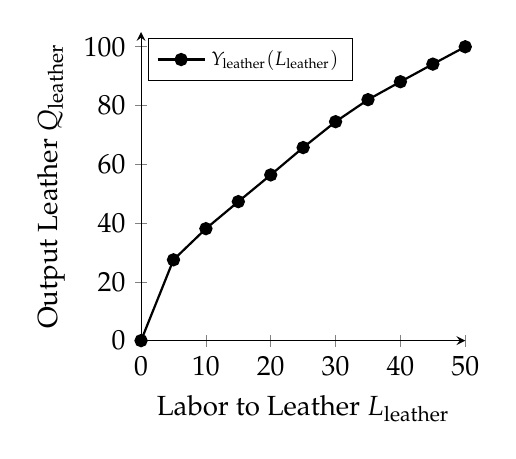
\begin{tikzpicture}
\begin{axis}[
    width=0.47\textwidth,height=5.5cm,
    axis lines=left, xlabel={Labor to Leather $L_{\text{leather}}$}, ylabel={Output Leather $Q_{\text{leather}}$},
    xmin=0,xmax=50,ymin=0,ymax=105, xtick={0,10,20,30,40,50}, ytick={0,20,40,60,80,100},
    legend style={at={(0.02,0.98)},anchor=north west, font=\scriptsize}
]
\addplot[thick, mark=*] table[row sep=\\]{
x y\\
0 0\\ 5 27.5\\ 10 38.1\\ 15 47.3\\ 20 56.4\\ 25 65.7\\ 30 74.5\\ 35 82.0\\ 40 88.1\\ 45 94.1\\ 50 100\\
};
\legend{$Y_{\text{leather}}(L_{\text{leather}})$}
\end{axis}
\end{tikzpicture}\hspace{8mm}
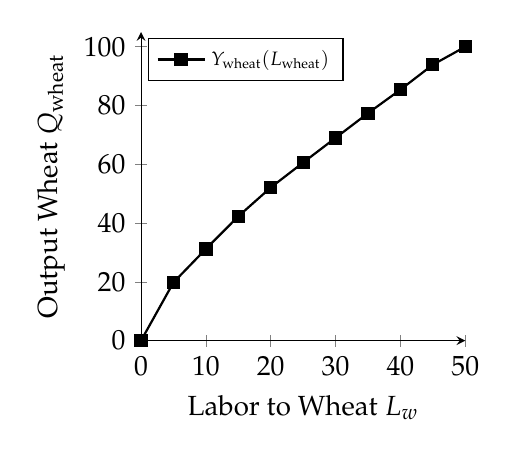
\begin{tikzpicture}
\begin{axis}[
    width=0.47\textwidth,height=5.5cm,
    axis lines=left, xlabel={Labor to Wheat $L_w$}, ylabel={Output Wheat $Q_{\text{wheat}}$},
    xmin=0,xmax=50,ymin=0,ymax=105, xtick={0,10,20,30,40,50}, ytick={0,20,40,60,80,100},
    legend style={at={(0.02,0.98)},anchor=north west, font=\scriptsize}
]
\addplot[thick, mark=square*] table[row sep=\\]{
x y\\
0 0\\ 5 19.8\\ 10 31.2\\ 15 42.3\\ 20 52.1\\ 25 60.6\\ 30 69.0\\ 35 77.4\\ 40 85.4\\ 45 93.9\\ 50 100\\
};
\legend{$Y_{\text{wheat}}(L_{\text{wheat}})$}
\end{axis}
\end{tikzpicture}
\end{center}

\part \textbf{Graph the PPF. What happens if more labor is employed?}

\textcolor{red}{The PPF is traced by $(Y_{\text{wheat}}(L_{\text{wheat}}),Y_{\text{leather}}(\bar L-L_{\text{wheat}}))$ for $L_{\text{wheat}}\in[0,\bar L]$. With more total labor $\bar L$, the PPF shifts outward (more of both goods at given prices).}

\medskip
\begin{center}
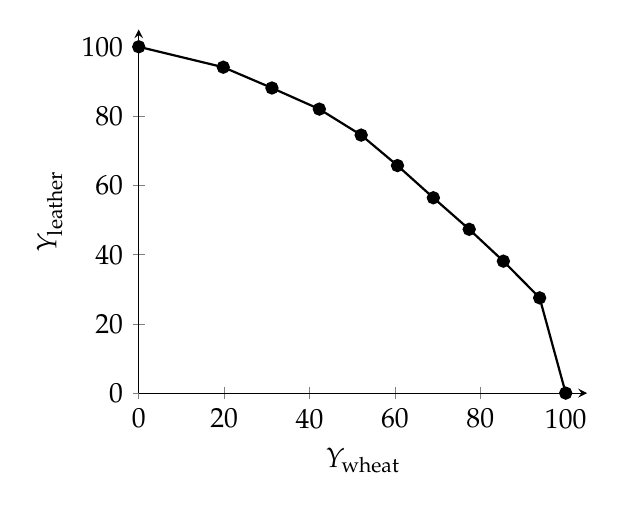
\begin{tikzpicture}
\begin{axis}[
    width=0.6\textwidth,height=6.2cm,
    axis lines=left, xlabel={$Y_{\text{wheat}}$}, ylabel={$Y_{\text{leather}}$},
    xmin=0,xmax=105,ymin=0,ymax=105, xtick={0,20,40,60,80,100}, ytick={0,20,40,60,80,100}
]
% parametric: step every 5 units of Lw
\addplot[thick, mark=*] coordinates
{ (0,100) (19.8,94.1) (31.2,88.1) (42.3,82.0) (52.1,74.5) (60.6,65.7)
  (69.0,56.4) (77.4,47.3) (85.4,38.1) (93.9,27.5) (100,0) };
\end{axis}
\end{tikzpicture}
\end{center}
\end{parts}

% ============================================================
\question The marginal product of labor curves corresponding to the production functions in problem 2 are as follows:

\begin{center}
\begin{tabular}{c c c}
\toprule
Workers employed (in a sector) & MPL in leather & MPL in wheat\\
\midrule
5 & 5.4 & 3.96\\
10& 2.3 & 2.28\\
15& 1.76& 2.22\\
20& 1.44& 1.96\\
25& 1.20& 1.74\\
30& 1.02& 1.62\\
35& 1.18& 1.60\\
40& 1.16& 1.46\\
45& 1.20& 1.54\\
50& 1.18& 1.38\\
\bottomrule
\end{tabular}
\end{center}

\begin{parts}
\part \textbf{Suppose the price of wheat relative to that of leather is 5. Determine the wage rate and the allocation of labor between the two sectors.}

\textcolor{red}{In the SFM, the common wage $w$ satisfies:
\begin{equation*}
w=P_{\text{leather}}\,\text{MPL}_{\text{leather}}(L_{\text{leather}})=P_{\text{wheat}}\,\text{MPL}_{\text{wheat}}(L_{\text{wheat}})
\end{equation*}
Since the relative price of wheat relative to leather is 5, then: $P_{\text{wheat}}/P_{\text{leather}} = 5$, which is the same as setting $P_{\text{wheat}} = 5, P_{\text{leather}} =1$.
}

\begin{center}
\begin{tabular}{r r r r c}
\toprule
$L_{\text{wheat}}$ & $L_{\text{leather}}$ 
& $P_{\text{wheat}}\!\cdot\!\text{MPL}_{\text{wheat}}$ & $P_{\text{leather}}\!\cdot\!\text{MPL}_{\text{leather}}$ & Comparison \\
\midrule
 5  & 45 & $5\!\times\!3.96=19.8$ & $1.20$ & $>$ \\
10  & 40 & $5\!\times\!2.28=11.4$ & $1.16$ & $>$ \\
15  & 35 & $5\!\times\!2.22=11.1$ & $1.18$ & $>$ \\
20  & 30 & $5\!\times\!1.96=9.8$  & $1.02$ & $>$ \\
25  & 25 & $5\!\times\!1.74=8.7$  & $1.20$ & $>$ \\
30  & 20 & $5\!\times\!1.62=8.1$  & $1.44$ & $>$ \\
35  & 15 & $5\!\times\!1.60=8.0$  & $1.76$ & $>$ \\
40  & 10 & $5\!\times\!1.46=7.3$  & $2.30$ & $>$ \\
45  & 5  & $5\!\times\!1.54=7.7$  & $5.40$ & $>$ \\
50  & 0  & $5\!\times\!1.38=6.9$  & $(n/a)$   & $>$ \\
\bottomrule
\end{tabular}
\end{center}

\textcolor{red}{
Using the discrete MPL schedules, for all feasible splits we have
\begin{equation*}
    P_{\text{wheat}}\,\text{MPL}_{\text{wheat}}(L_{\text{wheat}})>P_{\text{leather}}\text{MPL}_{\text{leather}}(L_{\text{leather}})
\end{equation*}
so there is \emph{no interior solution}. The allocation is a \textbf{corner}: all labor moves to the good with the higher value of marginal product, i.e.\ Sector 2 (wheat). Hence $L_{\text{wheat}}=50$, $L_{\text{leather}}=0$ and $w=P_{\text{wheat}}\text{MPL}_{\text{wheat}}(50)=5\times 1.38=6.9$.
}




% ============================================================
\question Consider two countries (Home and Foreign) that produce leather (with labor
and capital) and wheat (with labor and land) according to the production functions
described in problems 2 and 3. Initially, both countries have the same supply of
labor (100 units each), capital, and land. The capital stock in Home then grows.
This change shifts out both the production curve for good 1 as a function of labor employed (described in problem 2) and the associated marginal product of labor
curve (described in problem 3). Nothing happens to the production and marginal
product curves for good 2.

\begin{parts}
\part Show how the increase in the supply of capital for Home affects its production
possibility frontier.

\textcolor{red}{Home’s $Y_{\text{leather}}(L_{\text{leather}})$ shifts up for each $L_{\text{leather}}$; thus the PPF shifts outward, biased toward leather.}

\part If those two economies open up to trade, what will be the pattern of trade (i.e., which country exports which good)?

\textcolor{red}{Home becomes relatively abundant in the leather-specific factor (capital) and exports leather; Foreign exports wheat (the land-specific good).}

\part Describe how opening up to trade affects all three factors (labor, capital, land) in both countries.

\textcolor{red}{In Home: capital owners gain, landowners lose; wage effects are ambiguous but typically bounded between the two prices’ movements. In Foreign: landowners gain, capital owners lose.}
\end{parts}

\end{questions}

\end{document}